
\section{Framework Overview}\label{sec-arch}
In this section, we formalize the two main problems that \svc addresses: (1) cleaning a stale sample MV and (2) answering an aggregate query with the clean sample.

\subsection{Notation and Definitions}\label{notation}
\svc returns a bounded approximation for aggregate queries on stale MVs for a flexible additional maintenance cost.

%\reminder{You have defined $\mathcal{D}$, $\{R_i\}$, etc in Definition 1. Maybe you can move Def 1 to this Section?}
\noindent \textbf{Materialized View:} Let $\mathcal{D}$ be a database which is a collection of relations $\{R_i\}$. A \emph{materialized view} $S$ is the result of applying a \emph{view definition} to $\mathcal{D}$. 
View definitions are composed of standard relational algebra expressions: Select ($\sigma_{\phi}$), Project ($\Pi$), Join ($\bowtie$), Aggregation ($\gamma$), Union ($\cup$), Intersection ($\cap$) and Difference ($-$). 
We use the following parametrized notation for joins, aggregations and generalized projections:
\begin{itemize}[noitemsep] \sloppy
	\item $\Pi_{a_1,a_2,...,a_k}(R)$: Generalized projection selects attributes $\{a_1,a_2,...,a_k\}$ from $R$, allowing for adding new attributes that are arithmetic transformations of old ones (e.g., $a_1+a_2$).
	\item $\bowtie_{\phi (r1,r2)}(R_1,R_2)$: Join selects all tuples in $R_1 \times R_2$ that satisfy $\phi (r_1,r_2)$. We use $\bowtie$ to denote all types of joins even extended outer joins such as $\rightouterjoin,\leftouterjoin,\fullouterjoin$.
	\item $\gamma_{f,A}(R)$: Apply the aggregate function $f$ to the relation R grouped by the distinct values of $A$, where $A$ is a subset of the attributes.  
	The DISTINCT operation can be considered as a special case of the Aggregation operation. 
\end{itemize}
The composition of the unary and binary relational expressions can be represented as a tree, which is called the \emph{expression tree}.
The leaves of the tree are the \emph{base relations} for the view. 
Each non-leave node is the result of applying one of the above relational expressions to a relation.
To avoid ambiguity, we refer to tuples of the base relations as \emph{records} and tuples of derived relations as \emph{rows}.

\noindent \textbf{Primary Key:} We assume that each of the base relations has a \emph{primary key}. If this is not the case, we can always add an extra column 
that assigns an increasing sequence of integers to each record.
For the defined relational expressions, every row in a materialized view can also be given a primary key \cite{DBLP:journals/vldb/CuiW03, DBLP:conf/sigmod/ZengGMZ14},
which we will describe in Section \ref{sampling}. 
This primary key is formally a subset of attributes $u \subseteq \{a_1,a_2,...,a_k\}$ such that all $s \in S(u)$ are unique.

\vspace{.25em}

\noindent \textbf{Staleness:} For each relation $R_i$ there is a set of insertions $\Delta R_i$ (modeled as a relation)
and a set of deletions $\nabla R_i$.
An ``update'' to $R_i$ can be modeled as a deletion and then an insertion.
We refer to the set of insertion and deletion relations as ``delta relations", denoted by $\partial \mathcal{D}$:
\[
	\partial \mathcal{D} = \{\Delta R_1,...,\Delta R_k\} \cup \{\nabla R_1,...,\nabla R_k\}
\]
A view $S$ is considered \emph{stale} when there exist insertions or deletions to any of its base relations.
This means that at least one of the delta relations in $\partial \mathcal{D}$ is non-empty.

\vspace{.25em}

\noindent \textbf{Maintenance:} There may be multiple ways (e.g., incremental maintenance or recomputation) to maintain a view $S$, and we denote the up-to-date view as $S'$.
We formalize the procedure to maintain the view as a \emph{maintenance strategy} $\mathcal{M}$.
A maintenance strategy is a relational expression the execution of which will return $S'$.
It is a function of the database $\mathcal{D}$, the stale view $S$, and all the insertion and deletion relations $\partial \mathcal{D}$. 
In this work, we consider maintenance strategies composed of the same relational expressions as materialized views described above.
\[
S' = \mathcal{M}(S,\mathcal{D}, \partial D)
\]

\vspace{.25em}

\noindent \textbf{Staleness as Data Error:} The consequences of staleness are incorrect, missing, and superfluous rows. 
Formally, for a stale view $S$ with primary key $u$ and an up-to-date view $S'$:
\begin{itemize}[noitemsep] \sloppy
	\item \textbf{Incorrect: } Incorrect rows are the set of rows (identified by the primary key) that are updated in $S'$. For $s \in S$, let $s(u)$ be the value of the primary key. An incorrect row is one such that there exists a $s' \in S'$ with $s'(u) = s(u)$ and $s \ne s'$.
	\item \textbf{Missing: } Missing rows are the set of rows (identified by the primary key) that exist in the up-to-date view but not in the stale view. For $s' \in S'$, let $s'(u)$ be the value of the primary key. A missing row is one such that there does not exist a $s \in S$ with $s(u) = s'(u)$.
	\item \textbf{Superfluous: } Superfluous rows are the set of rows (identified by the primary key) that exist in the stale view but not in the up-to-date view. For $s \in S$, let $s(u)$ be the value of the primary key. A superfluous row is one such that there does not exist a $s' \in S'$ with $s(u) = s'(u)$.
\end{itemize}

\vspace{.25em}

\iffalse
\begin{figure}[t] \vspace{-2em}
\centering
 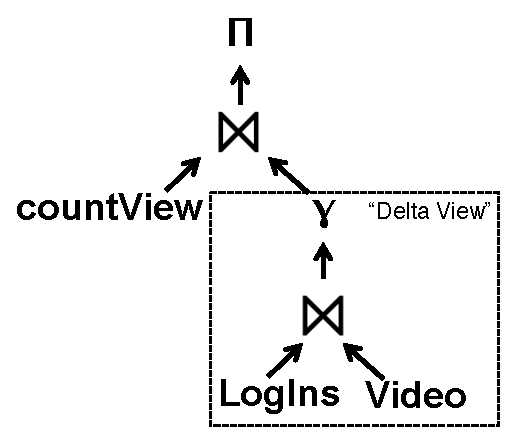
\includegraphics[scale=0.32]{figs/example_expression_tree.pdf} \vspace{-.5em}
 \caption{\reminder{(1). the view definition is different from the one in Sec 2.1; (2) Even if they are the same, it seems not necessary to show it again; (3) Right now you have (b) to show maintenance strategy; maybe you can replace (a) with a figure that shows primary key and ``staleness ad data error"} For our example, we represent the expression tree of the maintenance strategy. We first calculate a delta view using the new insertions and then join this view with the old view.\label{exexpr}}\vspace{-1.5em}
\end{figure}

\vspace{0.45em}
\fi

\noindent \textbf{Uniform Random Sampling:}
We define a sampling ratio $m\in [0,1]$ and for each row in a view $S$, we include it into a sample with probability $m$.
We use the ``hat'' notation (e.g., $\widehat{S}$) to denote sampled relations.
We say the relation $\widehat{S}$ is a \emph{uniform sample} of $S$ if
\[\text{(1) } \forall s \in \widehat{S} : s \in S\text{;~~~~~ (2) }Pr(s_1 \in \widehat{S}) =  Pr(s_2 \in \widehat{S}) = m.\]
We say a sample is \emph{clean} if and only if it is a uniform random sample of the up-to-date view $S'$. 

\vspace{0.25em}

\begin{example}\label{concepts}
In this example, we summarize all of the key concepts and terminology pertaining to materialized views, stale data error, and maintenance strategies.
Our example view, visitView, joins the Log table with the Video table and counts the visits for each video grouped by videoId.
Since there is a foreign key relationship between the relations, this is just a visit count for each unique video with additional attributes. 
The primary keys of the base relations are: sessionId for Log and videoId for Video.

If new records have been added to the Log table, the visitView is considered stale.
Incorrect rows in the view are videos for which the visitCount is incorrect and missing rows are videos that had not yet been viewed once at the time of materialization. 
While not possible in our running example, superfluous rows would be videos whose Log records have all been deleted.
Formally, in this example our database is $\mathcal{D}=\{Video, Log\}$, and the delta relations are $\partial\mathcal{D}=\{LogIns\}$. 

Suppose, we apply the change-table IVM algorithm proposed in~\cite{gupta1995maintenance}:
\vspace{-.55em}
\begin{enumerate}[noitemsep]
\item Create a ``delta view" by applying the view definition to LogIns. That is, calculate the visit count per video on the new logs:
\[
 \gamma(Video \bowtie LogIns)
\]
\item Take the full outer join of the ``delta view" with the stale view visitView (equality on videoId).
\[
 VisitView \fullouterjoin \gamma(Video \bowtie LogIns)
\]
\item Apply the generalized projection operator to add the visitCount in the delta view to each of the rows in visitView where we treat a NULL value as 0: 
\[
 \Pi (VisitView \fullouterjoin \gamma(Video \bowtie LogIns))
\]
Therefore, the maintenance strategy is:
\[
 \mathcal{M}(\{VisitView\},\{Video, Log\}, \{LogIns\})
\]
\[
\text{\hspace{0.7em}} = \Pi (VisitView \fullouterjoin \gamma(Video \bowtie LogIns))
\]
\end{enumerate}

\end{example}

%\begin{figure}[t] \vspace{-2em}
%\centering
% 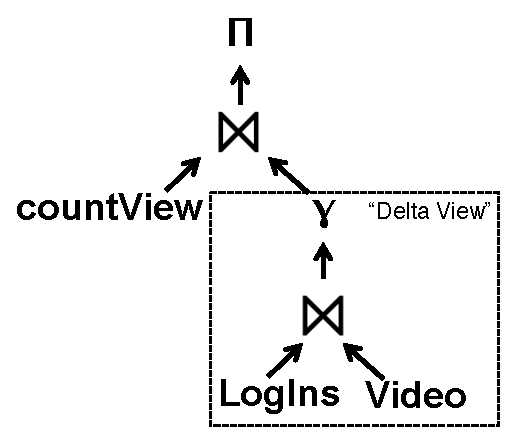
\includegraphics[scale=0.35]{figs/example_expression_tree.pdf} \vspace{-.5em}
% \caption{We illustrate the maintenance strategy of our example view, visitView, in an expression tree. \label{maintstrat}}\vspace{-1.75em}
%\end{figure}

%While, uniform sampling supports a wide variety of query types, it may have issues with queries with highly selective predicates.
%Stratfied sampling has been proposed to mitigate this problem as in the BlinkDB project \cite{AgarwalMPMMS13}.
%However, this requires that we know our query workload in advance.  
%In this paper, we do not discuss stratified sampling and will explore this further in future work.

\subsection{\svc Workflow}
%We summarize the system in Figure \ref{sys-arch} in our introduction.
Formally, the workflow of \svc is:
\begin{enumerate}[noitemsep]
\item We are given a view $S$.
\item $\mathcal{M}$ defines the maintenance strategy that updates $S$ at each maintenance period.
\item The view $S$ is stale between periodic maintenance, and the up-to-date view should be $S'$.
\item \emph{(Problem 1. Stale Sample View Cleaning)} We find an expression $\mathcal{C}$ derived from $\mathcal{M}$ 
that cleans a uniform random sample of the stale view $\widehat{S}$ to produce a ``clean" sample of the up-to-date
view $\widehat{S'}$.
\item \emph{(Problem 2. Query Result Estimation)} Given an aggregate query $q$ and the state query result $q(S)$, we use $\widehat{S'}$ and $\widehat{S}$ to estimate the up-to-date result.
\item We optionally maintain an index of outliers $o$ for improved estimation in skewed data.
\end{enumerate} 

\noindent\textbf{Stale Sample View Cleaning: }
The first problem addressed in this paper is how to clean a sample of the stale materialized view.
\begin{problem}[Stale Sample View Cleaning]
We are given a stale view $S$, a sample of this stale view $\widehat{S}$ with ratio $m$, the maintenance strategy $\mathcal{M}$, the base relations $\mathcal{D}$, and
the insertion and deletion relations $\partial \mathcal{D}$.
We want to find a relational expression $\mathcal{C}$ such that:
\[
\widehat{S}' = \mathcal{C}(\widehat{S},\mathcal{D},\partial \mathcal{D}),
\]
where $\widehat{S}'$ is a sample of the up-to-date view with ratio $m$. 
\end{problem}

\noindent\textbf{Query Result Estimation: }
The second problem addressed in this paper is query result estimation.
\begin{problem}[Query Result Estimation]
Let $q$ be an aggregate query of the following form \footnote{\scriptsize For simplicity, we exclude the group by clause for all queries in the paper, as it can be modeled as part of the \textsf{Condition}.}:
\begin{lstlisting} [mathescape,basicstyle={\scriptsize}]
SELECT $agg(a)$ FROM View WHERE Condition(A);
\end{lstlisting}
If the view $S$ is stale, then the result will be incorrect by some value~$c$:
\[
q(S') = q(S) + c
\]
Our objective is to find an estimator $f$ such that:
\[
q(S') \approx f(q(S),\widehat{S},\widehat{S}')
\] 
\end{problem}

\begin{example}\label{infexample}
Suppose a user wants to know how many videos have received more than 100 views.
\begin{lstlisting}[basicstyle={\scriptsize}]
SELECT COUNT(1) FROM visitView WHERE visitCount > 100;
\end{lstlisting}
Let us suppose the user runs the query and the result is $45$.
However, there have now been new records inserted into the Log table making this result stale. % (for clarity no changes to \tbl{Video} or deletions).
First, we take a sample of \tbl{visitView} and suppose this sample is a 5\% sample.
In Stale Sample View Cleaning (Problem 1), we apply updates, insertions, and deletions to the sample to efficiently materialize a 5\%  sample of the up-to-date view.
In Query Result Estimation (Problem 2), we estimate aggregate query results based on the stale sample and the up-to-date sample.
\end{example}

\iffalse
Our query correction component takes the two corresponding samples $\widehat{S'}$ and $\widehat{S}$, and calculates a correction to~$q(S)$.

Like similar restrictions in other sample-based systems \cite{agarwalknowing}, there are restrictions on the queries $q$ on the view that we can answer. 
In the SampleClean work, we focused on \sumfunc, \countfunc, and \avgfunc queries of the form\footnote{\scriptsize For simplicity, we exclude the group by clause for all queries in the paper, as it can be modeled as part of the \textsf{Condition}.}: 
\begin{lstlisting} [mathescape,basicstyle={\scriptsize}]
SELECT $f(a)$ FROM View WHERE Condition(A);
\end{lstlisting}
In this work, we expand the scope of the query processing, and consider general non-nested aggregate queries with predicates.

We also consider correcting stale non-nested select queries of the following form with predicates:
\begin{lstlisting} [mathescape,basicstyle={\scriptsize}]
SELECT * FROM View WHERE Condition(A);
\end{lstlisting}
As with all sample estimates, the accuracy increases with sample size, thus less selective predicates lead to more accurate results.




Note, that this definition is slightly different from the reservoir sampling techniques studied in AQP \cite{DBLP:journals/toms/Vitter85} which find a uniform sample of fixed \emph{size} $k\le \mid S \mid$.
Our sampling ratio gives a sample of the size $k$ in expectation, however, the actual size from any given instance may be slightly different.
For large sample sizes, there is little difference between the techniques since the actual size of using a sample ratio will be close to $k$.
The uniform sample model represents our algorithm which uses hashing better and also makes the presentation of our analysis more clear.

Furthermore, any ``black-box'' uniform sampling algorithm can be used to achieve a reservoir sample.
The use of one technique over another does not affect the general principles or the statistics of \svc, only the 
notation in the analysis.


%\vspace{2em}
\subsection{Problem Statements}
\subsubsection{View Maintenance as Data Cleaning}\label{cleaning}
%In \svc, we model staleness in an MV as a type of data error.
We formalize the problem of correcting staleness as a data cleaning operation so we can apply our data cleaning approach.
In the unsampled case, $\mathcal{M}$ defines a data cleaning operation.
If we are given a materialized view $S$ and we know the base relations have had insertions and deletions, then there are three possible types of error:
(1) a row in $S$ needs to be updated, (2) a row in $S$ needs to be deleted, and (3) new row needs to be inserted into $S$.
Applying $\mathcal{M}$ removes these errors making the view ``clean".
%In the absence of these errors, we call a view \emph{up-to-date}.

However, now suppose we have a sampled view $\widehat{S}$, simply applying updates to the rows in the sample may not suffice.
If new rows need to be inserted into $S$, those will never be represented in the sample violating our uniform sampling.
Thus, we define cleaning in the following way: suppose we have a stale uniform sample $\widehat{S}$, cleaning this sample
should give us $\widehat{S'}$ a uniform sample of the up-to-date view $S'$ with the same sampling ratio.
Formally, this can be represented as the following operations: (1) if an update is needed, update the row, (2) if a row needs to be deleted, delete the row, and (3) for all new rows that need to be inserted into the view $S$ insert a random sample of ratio $m$.

Due to the insertions, the defined data cleaning on a sample does not necessarily give a unique $\widehat{S'}$, so the next question is how to formalize the link between $\widehat{S}$ and $\widehat{S'}$. 
To link a corresponding stale sample (dirty data) and up-to-date sample (clean data), we define the following property:
\begin{definition}[Correspondence]
$\widehat{S'}$ and $\widehat{S}$ are uniform samples of $S'$ and $S$, respectively.  We say $\widehat{S'}$ and $\widehat{S}$ correspond if and only if:
\vspace{-.25em}
\begin{itemize}[noitemsep]
\item For every row $r$ in $\widehat{S}$ that required a delete, $r \not\in \widehat{S'}$
\item For every row $r$ in $\widehat{S}$ that required an update to $r'$, $r' \in \widehat{S'}$
\item For every row $r$ in $\widehat{S}$  that was unchanged, $r \in \widehat{S'}$
\item For every row $r$ in $S$ but not in $\widehat{S}$, $r \not\in \widehat{S'}$
\end{itemize}
\vspace{-.25em}
%\item For every row $r$ in $S'$ that is newly inserted, $r \not\in \widehat{S}$.
%\item If a row $r$ requires an update and then a deletion. The deletion takes precedence and $r \not\in \widehat{S'}$.
%\item Rows that are inserted trivially satisfy the conditions since those rows are not contained in $S$ or $\widehat{S}$.
\label{correspondence}
\end{definition}
%This definition of correspondence gives us a way to get two samples from which we can take a row-by-row difference.
%There is some nuance in how to handle null values which we discuss in Section \ref{correction}.

The goal of \svc is to efficiently produce a corresponding up-to-date sample from a stale one thus cleaning the sample.
In the first component of \svc (Section \ref{sampling}), we take as input a uniform sample of a stale view $\widehat{S}$, a maintenance strategy $\mathcal{M}$, and a set of updates $\{\Delta R_i\} \cup \{\nabla R_i\}$.
We return $\widehat{S'}$, a clean uniform sample (a uniform sample of $S'$) that satisfies the correspondence property with $\widehat{S}$.

\iffalse

\begin{example}[Correspondence]
Suppose \tbl{countView} has 4 video rows: 
\begin{lstlisting} [mathescape]
V1 (visitCount = 4), V2 (visitCount = 6), V3 (visitCount = 1), V4 (visitCount = 1)
\end{lstlisting}
We take a sample of \tbl{countView} and call it \tbl{countViewSample} that contains V1 and V2.
\tbl{LogIns} has new logs of 1 visit for V1 and 1 visit for a new video V5.
An up-to-date sample that corresponds is:
\begin{lstlisting} [mathescape]
V1 (visitCount = 4+1), V2 (visitCount = 6)
\end{lstlisting}
An up-to-date sample that does \emph{not} corresponds is: 
\begin{lstlisting} [mathescape]
V1 (visitCount = 4+1), V3 (visitCount = 1)
\end{lstlisting}
This is because V2 was unchanged and therefore should be included in the sample.
\end{example}
\fi

\subsubsection{Query Result Correction}
In the query result correction phase, we take a query result on a stale view and use the up-to-date sample to compensate for the staleness.
Given a query $q$ which has been applied to the stale view $q(S)$ giving a stale result.
Our query correction component takes the two corresponding samples $\widehat{S'}$ and $\widehat{S}$, and calculates a correction to~$q(S)$.

Like similar restrictions in other sample-based systems \cite{agarwalknowing}, there are restrictions on the queries $q$ on the view that we can answer. 
In the SampleClean work, we focused on \sumfunc, \countfunc, and \avgfunc queries of the form\footnote{\scriptsize For simplicity, we exclude the group by clause for all queries in the paper, as it can be modeled as part of the \textsf{Condition}.}: 
\begin{lstlisting} [mathescape,basicstyle={\scriptsize}]
SELECT $f(a)$ FROM View WHERE Condition(A);
\end{lstlisting}
In this work, we expand the scope of the query processing, and consider general non-nested aggregate queries with predicates.

We also consider correcting stale non-nested select queries of the following form with predicates:
\begin{lstlisting} [mathescape,basicstyle={\scriptsize}]
SELECT * FROM View WHERE Condition(A);
\end{lstlisting}
As with all sample estimates, the accuracy increases with sample size, thus less selective predicates lead to more accurate results.
%From these queries, we exclude the group by clause, as we model group by clauses as part of the \textsf{Condition}.
\fi

\iffalse
\subsubsection{Outlier Indexing}
The query correction in the previous subsection is derived from a sample.
Sampling is known to be sensitive to outliers, which we define as records whose values deviate significantly from the mean.
However, a challenge is that since we do not materialize the entire up-to-date view detecting which records may be outliers is challenging.
Instead, we define an outlier index on base relations of the database $\mathcal{D}$.
This index tracks records whose attributes cross some threshold $t$.
Then, for a given view $S$, this component gives a series of rules to propagate the information from the outlier index upwards.
Basically, for every row in the view that is derived from a record in the outlier index, we ensure that it is incorporated into the sample.
We use the set of outliers to return a more accurate correction result.
\fi
%We explore the conditions under which we can make this guarantee, and discuss query processing with the outlier index in Section \ref{outlier}.


\iffalse
\subsection{Example Application}
Returning to our example \tbl{countView}, suppose a user wants to know how many videos have received more than 100 views.
\begin{lstlisting}[basicstyle={\scriptsize}]
SELECT COUNT(1) FROM visitView 
WHERE visitCount > 100;
\end{lstlisting}
Let us suppose the initial query result is $45$.
There now have been new log records inserted into the Log table making the old result stale.
For example, if our sampling ratio is 5\%, that means for 5\% of the videos (distinct \tbl{videoId}), we update just the view counts of those videos.
Suppose 2 videos have changed their counts from less than 100 to greater than 100.
%From this sample, we calculate how many new videos changed from less than 100 views to times greater than 100; let us suppose this answer is $2$.
%Since our sampling ratio is 5\%, 
From this sample, we extrapolate that $40$ new videos throughout the view should now be included in the count.
This means that we should correct the old result by $40$ resulting in the estimate of $45+40 = 85$.
\fi

